\documentclass[a4paper,twoside,12pt]{mgr}
\makeatletter
\def\@cite#1#2{{#1\if@tempswa , #2\fi}}
\makeatother
\usepackage{fancyhdr}
\pagestyle{fancy}
\usepackage{cite}
\usepackage{polski}
\usepackage[utf8]{inputenc}
\usepackage{float}
\restylefloat{figure}
\usepackage{listingsutf8}
\usepackage{color}
\usepackage{textcomp}
\definecolor{listinggray}{gray}{0.9}
\definecolor{lbcolor}{rgb}{0.9,0.9,0.9}

\lstset{
    inputencoding=utf8,
	backgroundcolor=\color{lbcolor},
	tabsize=4,
	rulecolor=,
	language=java,
        basicstyle=\scriptsize,
        upquote=true,
        aboveskip={1.5\baselineskip},
        columns=fixed,
        showstringspaces=false,
        extendedchars=true,
        breaklines=true,
        prebreak = \raisebox{0ex}[0ex][0ex]{\ensuremath{\hookleftarrow}},
        frame=single,
        showtabs=false,
        showspaces=false,
        showstringspaces=false,
        identifierstyle=\ttfamily,
        keywordstyle=\color[rgb]{0,0,1},
        commentstyle=\color[rgb]{0.133,0.545,0.133},
        stringstyle=\color[rgb]{0.627,0.126,0.941},
}
\usepackage{graphicx}
\fancyhf{}
\fancyhead[LE,LO]{\leftmark}
\fancyfoot[CE,CO]{- \thepage\ -}
%\linespread{1.3}
\fancypagestyle{plain}{
\fancyhead[LE,LO]{\leftmark}
\fancyfoot[CE,CO]{- \thepage\ -} 
}
\raggedbottom


%**************************************************************************
% Dane do strony tytułowej
%

% Autor
\autor{Piotr Zyszczak, Damian Łukasik}

% Rodzaj pracy - wpisać LICENCJACKA, INŻYNIERSKA lub MAGISTERSKA
\rodzajPracy{}

% Tytuł pracy magisterskiej/inżynierskiej
\tytul{Active Directory Windows 2008 Server – zasady budowy bezpiecznego środowiska}

% Rok
\rok{2015}

% Kierunek
\kierunek{Informatyka}

% Studia stacjonarne lub niestacjonarne (wpisać jakie)
\studia{stacjonarne}

% Poziom studiów wpisać I lub II
\poziomStudiow{II}


% Numer albumu
\numerAlbumu{113066/112993}

%
%**************************************************************************


% Styl dla wtrąceń anglojęzycznych
\newcommand{\eng}[1]{(\emph{#1})}

\begin{document}

\stronaTytulowa

\tableofcontents
\chapter{Cel i zakres zajęć}
Zainstalować maszynę wirtualną windows server 2008 a na niej zainstalować i skonfigurować:
\begin{itemize}
\item Active Directory
\item Domenę
\item Serwer DNS
\item Usługi routingu i dostępu zdalnego
\end{itemize}

\chapter{Wstęp teoretyczny}
Active Directory, AD – usługa katalogowa (hierarchiczna baza danych) dla systemów Windows – Windows Server 2012, Windows Server 2008, Windows Server 2003 oraz Windows 2000, będąca implementacją protokołu LDAP.

W Active Directory informacje grupowane są hierarchicznie. Podstawową jednostką jest tzw. liść, który położony jest w kontenerze w Active Directory nazywanym jednostką organizacyjną (ang. organizational unit, OU). Liście i kontenery zorganizowane są w domeny.

Drzewo

Domeny zorganizowane hierarchicznie mogą tworzyć strukturę drzewa. Drzewo posiada zawsze przynajmniej jedną domenę – domenę najwyższego poziomu (ang. root) – korzeń drzewa. Pozostałe domeny (o ile istnieją) mogą być umieszczone poniżej domeny najwyższego poziomu, tworząc drzewo. Niższe poziomy mogą się rozgałęziać.

Las

Każde drzewo jest w lesie(ang. the forest). Las składa się z przynajmniej jednego drzewa. Nie istnieje możliwość utrzymywania drzewa bez utrzymywania lasu. Uwaga ta odnosi się również do domeny Active Directory – domena nie może istnieć samodzielnie, musi istnieć w jakimś drzewie i jakimś lesie. Jeżeli jest to pierwsza domena, to tworzy pierwsze drzewo (którego korzeniem się staje) oraz pierwszy las. Las bierze nazwę od tej domeny.

Domena internetowa – ciąg nazw systemu Domain Name System (DNS) wykorzystywany w Internecie, składający się z wyrazów umieszczonych w pewnym poddrzewie struktury DNS tj. zakończonych stałym sufiksem (np. ".wikipedia.org").
Domena internetowa składa się z dwóch części - nazwy głównej oraz końcówki - rozszerzenia. Nazwę główną bardzo często tworzy nazwa firmy/organizacji/akcji jej skrót, bądź nazwa działalności, którą dana firma wykonuje. Rozszerzenie jest odgórnie ustalone - można wybrać spośród możliwych propozycji. Każdy kraj posiada przypisane rozszerzenie np. Polska - .pl, Rosja - .ru, Niemcy - .de, dla krajów Unii Europejskiej - .eu itd. Rozróżniamy domeny najwyższego poziomu: .com, .net, .org. Do tego pojawiają się rozszerzenia powstałe dla odróżnienia celu strony - lista domen najwyższego poziomu.
Od stycznia 2014 roku pojawiły się nowe rozszerzenia (ok. 700 końcówek) tzw. nowe domeny. Dzięki nowym domenom jest możliwość stworzenia krótkiej, chwytliwej nazwy domeny bez historii. Dla przykładu nowe domeny to .hotel, .blog, .fitness, .bar etc. Wdrożenie wszystkich końcówek zajęło cały rok 2014. Pierwszym największym rejestratorem nowych domen w Polsce była spółka Domeny.pl Sp. z o.o.

Adres, jaki jest wpisywany w przeglądarkę, a konkretnie jego część związana z domeną, musi zostać przetłumaczony na numer IP, pod którym nasłuchuje serwer WWW (czy FTP). Tłumaczenia tego dokonuje serwer DNS.
DNS jest zatem usługą drugoplanową, ale bez niej korzystanie z hostingu (czy komunikacja w Internecie w ogóle) będzie bardzo utrudniona. Dlatego też udostępniamy swoim klientom przynajmniej trzy takie serwery pracujące na różnych maszynach. 

Trasowanie (ang. routing, ruting, rutowanie) – wyznaczanie trasy i wysłanie nią pakietu danych w sieci komputerowej. Urządzenie węzłowe, w którym kształtowany jest ruch sieciowy, nazywane jest routerem – jego rolę może pełnić np. komputer stacjonarny czy oddzielne dedykowane urządzenie.
Pakiety przesyłane przez sieć opatrzone są adresem nadawcy i odbiorcy. Zadaniem routerów jako węzłów pośrednich między nadawcą a odbiorcą jest przesłanie pakietów do celu po jak najlepszej ścieżce. Typowy router bierze pod uwagę tylko informacje z nagłówka IP, czyli sprawdza tylko informacje z warstwy sieci (trzeciej) modelu OSI. Obowiązkiem routera IP przy przekazywaniu pakietu dalej do celu jest obniżenie o jeden wartości TTL (ang Time To Live, czas życia). Datagram IP, który trafia do routera z wartością 1 (a zostanie ona zmniejszona na tym routerze do 0) w polu TTL zostanie utracony, a do źródła router odsyła datagram ICMP z kodem TTL Exceeded.
Routery utrzymują tablice trasowania, na podstawie których kierują pakiety od określonych nadawców do odbiorców, bądź kolejnych routerów. Tablica może być budowana statycznie (trasowanie statyczne) lub dynamicznie (protokoły trasowania dynamicznego, takie jak RIP, IGRP, EIGRP, OSPF, BGP, IS-IS).
Trasowanie ma na celu możliwie najlepiej (optymalnie) dostarczyć pakiet do celu. Pierwotnie jedynym kryterium wyboru było posiadanie jak najdokładniejszej trasy do celu, ale obecnie protokoły trasowania mogą uwzględniać podczas wyboru trasy również takie parametry jak priorytet pakietu (standardy ToS/DSCP), natężenie ruchu w poszczególnych segmentach sieci itp. W przypadku trasowania brzegowego (wykorzystującego BGP) w Internecie wybór trasy jest silnie związany z polityką poszczególnych dostawców (i zawartymi między nimi umowami o wymianie ruchu) i bywa daleki od optymalnego.
Popularnym algorytmem służącym do wyznaczania tras w sieciach wewnętrznych jest algorytm Dijkstry wyznaczania najkrótszej ścieżki w grafie (np. OSPF).

\chapter{Przebieg}
Pierwszym etapem było zainstalowanie na VirtualBox-ie wirtualnej maszyny z systemem windows dla serwerów dostarczonemu przez prowadzącego.

\begin{figure}[H]
\centering
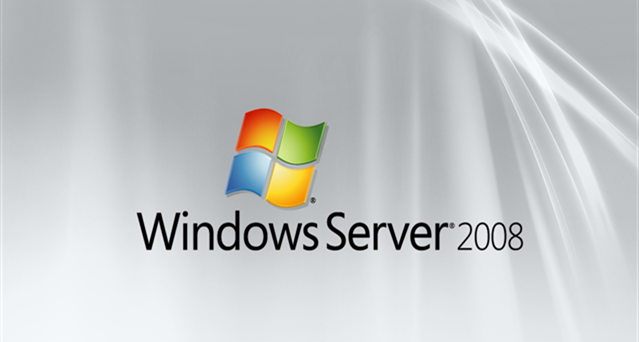
\includegraphics[scale=0.70]{winlogo.png}
\caption{System serwera.}%
\label{rys:etykieta}
\end{figure} 

W maszynie wirtualnej trzeba było ustawić karty sieciowe na 1- Bridget Adapter dla serwera i 2- NAT- dla klienta. 

Następnie należało zainstalować AD na maszynie wirtualnej pełniącej rolę serwera (w odpowiedniej zakładce w manadżerze jeśli chcemy dodać nową rolę dla servera powinna wyświetlić się nam lista a w niej Active directory). Dla poprawnego działania powinno się ustawić stałe ip przykłądowe ustawienie, dla TCP/IPv4:
IP Adress: 192.168.12.1
Maska podsieci: 255.255.255.0
Należało również wyłączyć zaporę systemu Windows.

W Menedżerze serwera (zakładka role) dodaliśmy rolę „Active Directory Domain Services”. Po udanej instalacji uruchomiony został serwer w trybie kontrolera domeny. Program dcpromo.exe . Wówczas pojawia się kreator instalacji usług domenowych. Tworzymy nową domenę w nowym lesie, a na nazwę nowej domeny przypisujemy frazę wybraną przez nas zgodną z poleceniem w oknie.

Jako dodatkowe opcje dla kontrolera domeny:
\begin{itemize}
\item Serwer DNS (by usługa działała)
\item Dynamicznie przydzielane adresy IP
\item Lokalizacja bazy danych, plików dziennika oraz folderu SYSVOL: Domyślne
\item Ustawiamy hasło konta administratora trybu przywracania usług domenowych 
\end{itemize}

Po zaakceptowaniu zmian należy ponownie uruchomić wirtualkę.

Kolejnym etapem było dodanie użtkowników.
Menedżer Serwera-> Role-> Active Directory Domain Services->laboratorium.pl-> Users -> New Users

Mając dodanych użytkowników, należało dołączyć ich do domeny. Komputer->właściwości->zmiana nazwy komputera/domeny->opcja Domena (laboratorium.pl) -> wpisujemy nazwy użytkowników i hasła. Komputer zostaje podłączony do naszej domeny .

Kolejnym zadaniem była instalacja roli usług zasad sieciowych oraz dostępu sieciowego.
Menedżer Serwera -> Role -> Dodaj rolę -> Network Policy and Access Services -> W kolejnym okienku wybiera się opcje:
\begin{itemize}
\item Routing and Remote Access Services
\item Remote Access Service
\item Routing
\end{itemize}

Kolejne ponowne uruchomienie.

Dalej należy skonfigurować dostęp zdalny.
Menedżer serwera-> Routing and Remote Access-> Konfiguruj i włącz routing i dostęp zdalny -> Network Address Translation (NAT) (Translator adresów sieciowych) -> Dalej-> Wirtualna karta sieciowa (obszar lokalny) -> Otrzymujemy powiadomienie, że serwer usług sieciowych został skonfigurowany.

\chapter{Wnioski}
Na laboratorium zostały zrealizowane wszystkie 4 postawione przed zespołem zadania. Skonfigurowano server i przetestowano jego działanie.

\end{document}
